\documentclass{article}
\usepackage{amsmath,amssymb,amsthm,mdframed,kotex,paralist}
\usepackage{tabto}
%\TabPositions{0.5\textwidth}
\TabPositions{0.33\textwidth,0.66\textwidth}
\newcommand\bp[1]{\begin{mdframed}[frametitle={#1},skipabove=10pt,skipbelow=20pt,innertopmargin=5pt,innerbottommargin=40pt]}
\newcommand\ep{\end{mdframed}\par}
\newcommand\ov[1]{\ensuremath{\overline{#1}}}
\newcounter{sqrt}
\newcommand\sqr{\stepcounter{sqrt}\item\(\sqrt{\thesqrt}\)}

\begin{document}
\title{영석01-삼각비 문제(1)}
\author{}
\date{\today}
\maketitle

\section{간단한 근호의 계산}
\bp{01}
다음을 간단히 하시오.
\begin{enumerate}[(1)]
\sqr\sqr\sqr\sqr\sqr\sqr\sqr\sqr\sqr\sqr\sqr\sqr\sqr\sqr\sqr\sqr\sqr\sqr\sqr\sqr
\sqr\sqr\sqr\sqr\sqr\sqr\sqr\sqr\sqr\sqr\sqr\sqr\sqr\sqr\sqr\sqr\sqr\sqr\sqr\sqr
\sqr\sqr\sqr\sqr\sqr\sqr\sqr\sqr\sqr\sqr\sqr\sqr\sqr\sqr\sqr\sqr\sqr\sqr\sqr\sqr
\sqr\sqr\sqr\sqr\sqr\sqr\sqr\sqr\sqr\sqr\sqr\sqr\sqr\sqr\sqr\sqr\sqr\sqr\sqr\sqr
\sqr\sqr\sqr\sqr\sqr\sqr\sqr\sqr\sqr\sqr\sqr\sqr\sqr\sqr\sqr\sqr\sqr\sqr\sqr\sqr
\end{enumerate}
\ep

\section{간단한 이차방정식}
\bp{02}
다음 이차방정식들의 근을 구하시오.
\begin{enumerate}[(1)]
\item\(x^2={0}\)
\item\(x^2={4}\)
\item\(x^2={8}\)
\item\(x^2={9}\)
\item\(x^2={12}\)
\item\(x^2={15}\)
\item\(x^2={20}\)
\item\(x^2={24}\)
\item\(x^2={30}\)
\item\(x^2={45}\)
\end{enumerate}
\ep

\bp{02}
다음 식을 만족하는 \(x\)를 구하시오. (단 \(x>0\))
\begin{enumerate}[(1)]
\item\(x^2={3}\)
\item\(x^2={5}\)
\item\(x^2={6}\)
\item\(x^2={7}\)
\item\(x^2={18}\)
\item\(x^2={28}\)
\item\(x^2={42}\)
\item\(x^2={48}\)
\item\(x^2={50}\)
\end{enumerate}
\ep


\section{간단한 피타고라스의 정리}
\bp{03}
다음 그림에서 \ov{BC}의 길이는?
\par\center
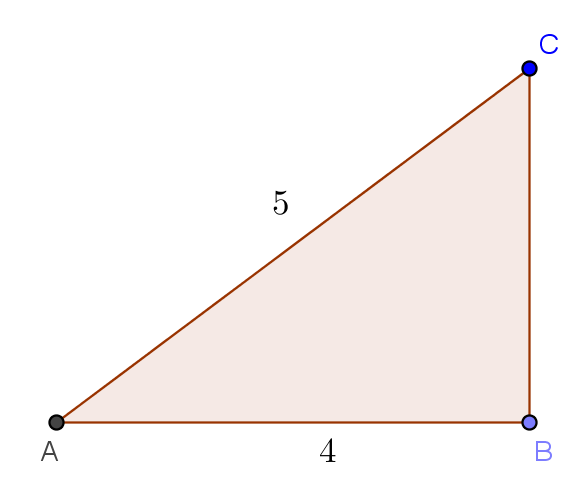
\includegraphics[width=0.3\textwidth]{03}
\ep

\bp{04}
다음 그림에서 \ov{AC}의 길이는?
\par\center
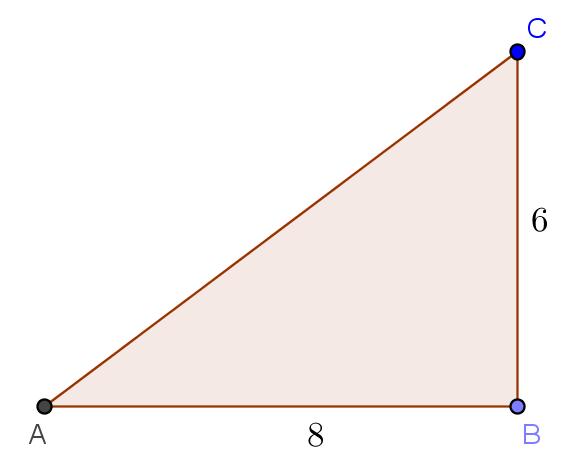
\includegraphics[width=0.3\textwidth]{04}
\ep

\bp{05}
다음 그림에서 \ov{BC}의 길이는?
\par\center
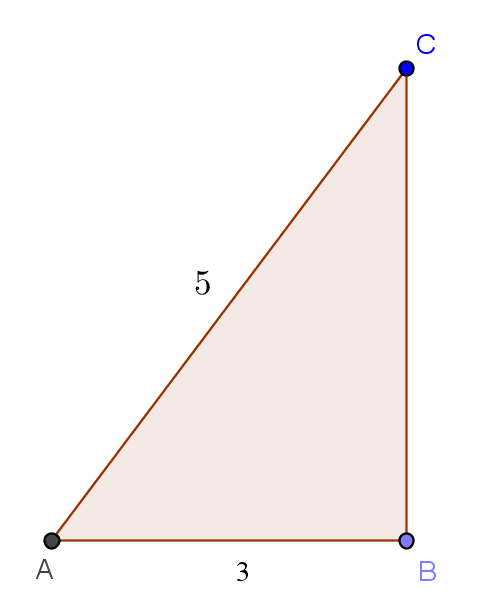
\includegraphics[width=0.3\textwidth]{05}
\ep

\bp{06}
다음 그림에서 \ov{AC}의 길이는?
\par\center
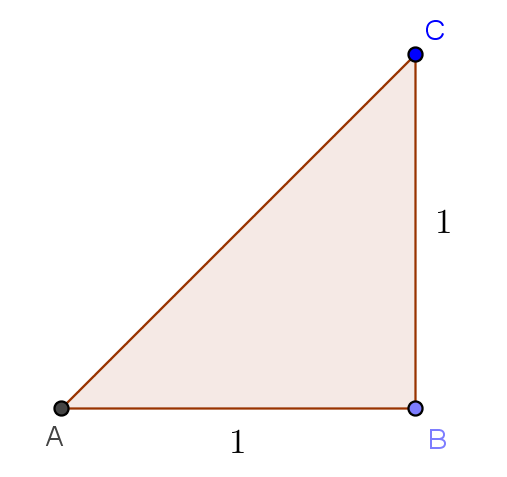
\includegraphics[width=0.3\textwidth]{06}
\ep

\bp{07}
다음 그림에서 \ov{AC}의 길이는?
\par\center
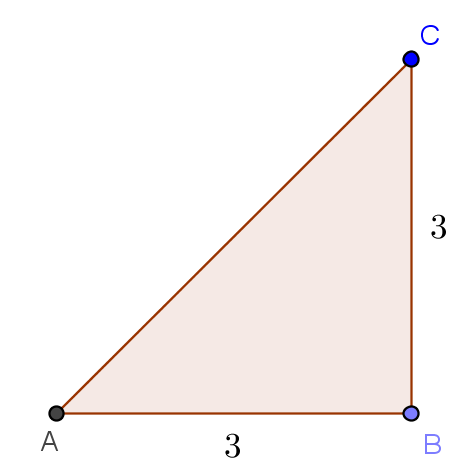
\includegraphics[width=0.3\textwidth]{07}
\ep


\bp{08}
다음 그림에서 \ov{AB}의 길이는?
\par\center
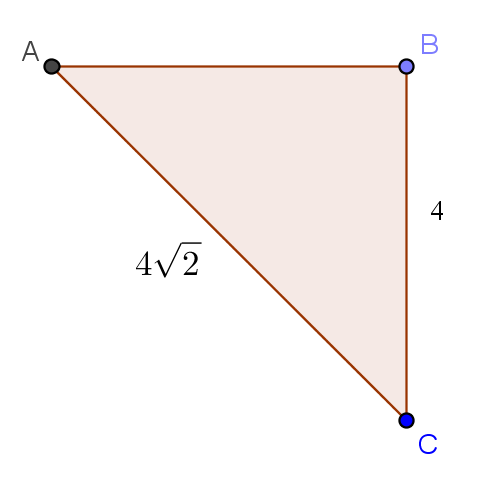
\includegraphics[width=0.3\textwidth]{08}
\ep

\bp{09}
다음 그림에서 \ov{AC}의 길이는?
\par\center
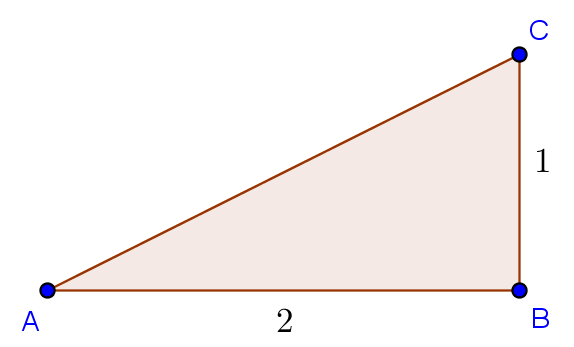
\includegraphics[width=0.3\textwidth]{09}
\ep

\bp{10}
다음 그림에서 \ov{AC}의 길이는?
\par\center
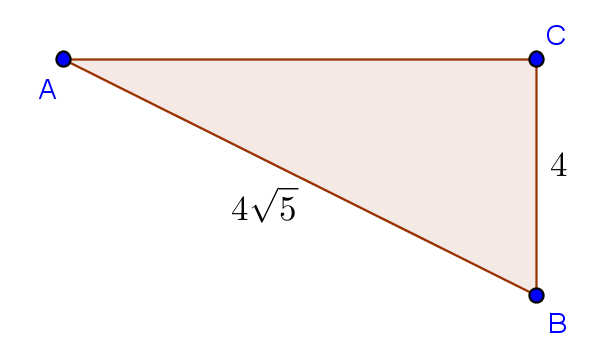
\includegraphics[width=0.3\textwidth]{10}
\ep

\bp{11}
다음 그림에서 \ov{AB}의 길이는?
\par\center
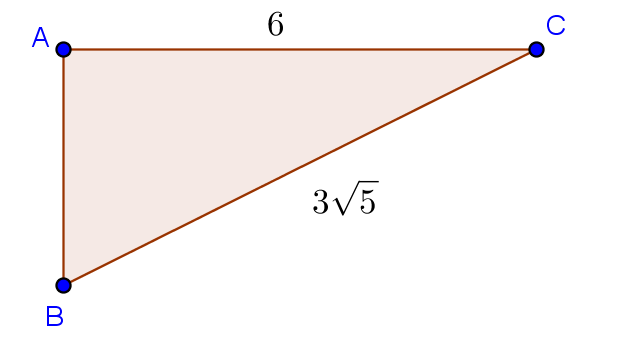
\includegraphics[width=0.3\textwidth]{11}
\ep

\bp{12}
다음 그림에서 \ov{AC}의 길이는?
\par\center
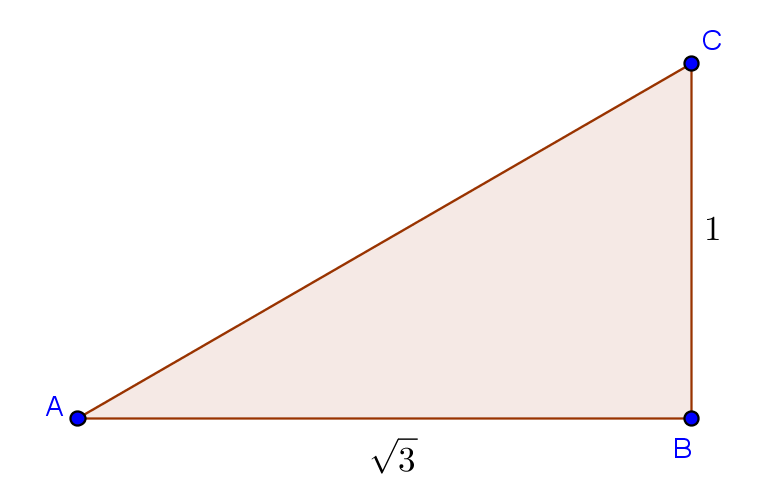
\includegraphics[width=0.3\textwidth]{12}
\ep

\bp{13}
다음 그림에서 \ov{BC}의 길이는?
\par\center
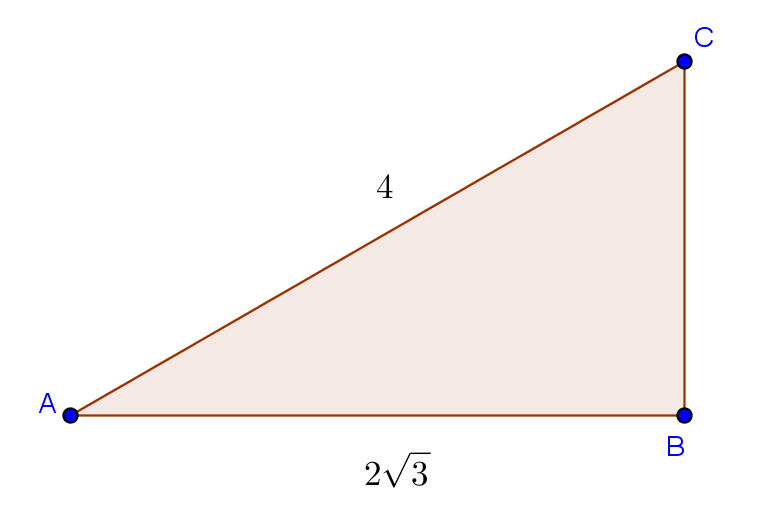
\includegraphics[width=0.3\textwidth]{13}
\ep

\bp{14}
다음 그림에서 \ov{AB}의 길이는?
\par\center
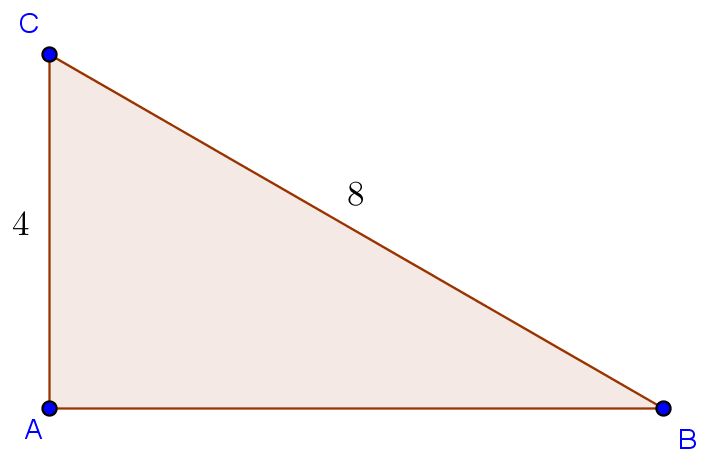
\includegraphics[width=0.3\textwidth]{14}
\ep

\section{간단한 삼각비 문제}
\bp{15}
다음 그림의 삼각형에서 \(\angle A\)의 삼각비를 각각 구하여라.\\
(1) \(\sin A\) =\\
(2) \(\cos A\) =\\
(3) \(\tan A\) =
\par\center
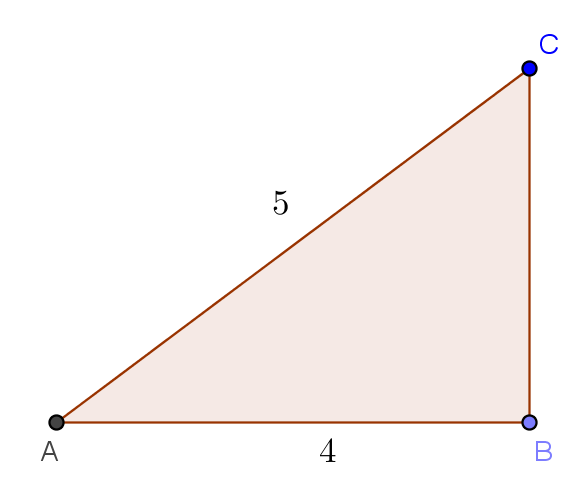
\includegraphics[width=0.3\textwidth]{03}
\ep

\bp{16}
다음 그림의 삼각형에서 \(\angle A\)의 삼각비를 각각 구하여라.\\
(1) \(\sin A\) =\\
(2) \(\cos A\) =\\
(3) \(\tan A\) =
\par\center
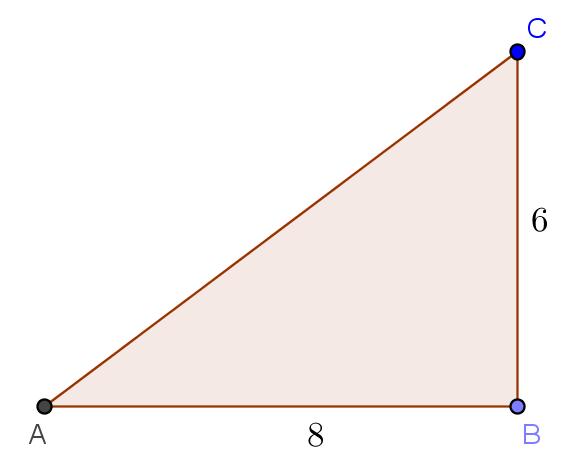
\includegraphics[width=0.3\textwidth]{04}
\ep

\bp{17}
다음 그림의 삼각형에서 \(\angle A\)의 삼각비를 각각 구하여라.\\
(1) \(\sin A\) =\\
(2) \(\cos A\) =\\
(3) \(\tan A\) =
\par\center
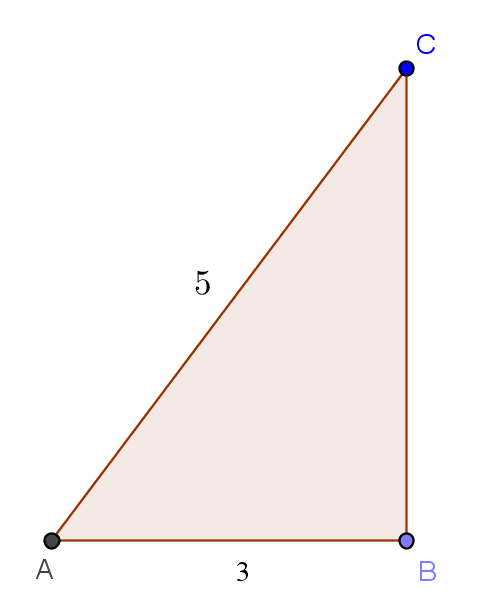
\includegraphics[width=0.3\textwidth]{05}
\ep

\bp{18}
다음 그림의 삼각형에서 \(\angle A\)의 삼각비를 각각 구하여라.\\
(1) \(\sin A\) =\\
(2) \(\cos A\) =\\
(3) \(\tan A\) =
\par\center
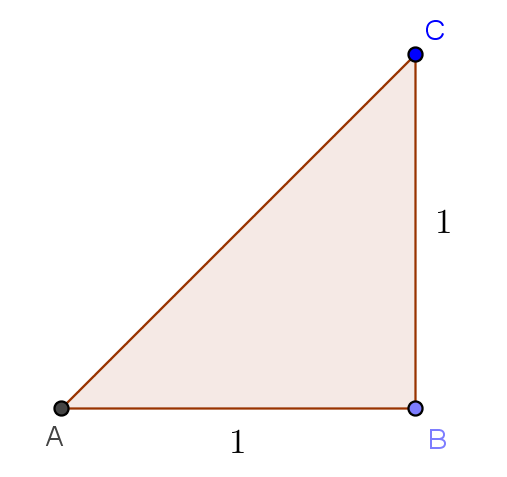
\includegraphics[width=0.3\textwidth]{06}
\ep

\bp{19}
다음 그림의 삼각형에서 \(\angle A\)의 삼각비를 각각 구하여라.\\
(1) \(\sin A\) =\\
(2) \(\cos A\) =\\
(3) \(\tan A\) =
\par\center
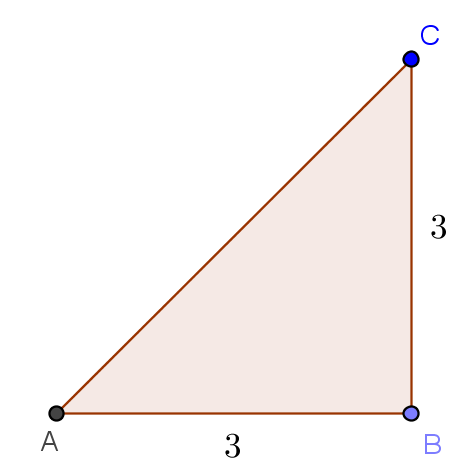
\includegraphics[width=0.3\textwidth]{07}
\ep

\bp{20}
다음 그림의 삼각형에서 \(\angle A\)의 삼각비를 각각 구하여라.\\
(1) \(\sin A\) =\\
(2) \(\cos A\) =\\
(3) \(\tan A\) =
\par\center
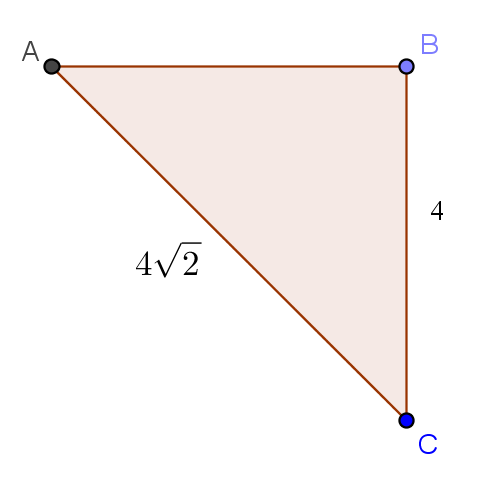
\includegraphics[width=0.3\textwidth]{08}
\ep

\bp{21}
다음 그림의 삼각형에서 \(\angle A\)의 삼각비를 각각 구하여라.\\
(1) \(\sin A\) =\\
(2) \(\cos A\) =\\
(3) \(\tan A\) =
\par\center
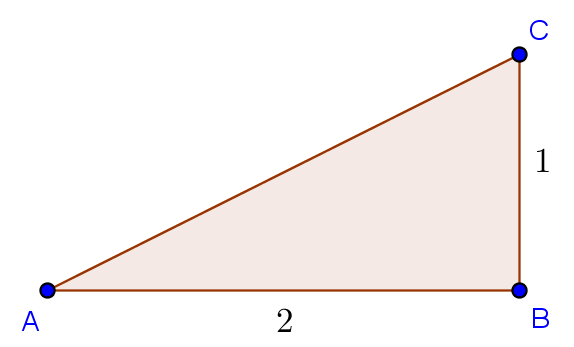
\includegraphics[width=0.3\textwidth]{09}
\ep

\bp{22}
다음 그림의 삼각형에서 \(\angle A\)의 삼각비를 각각 구하여라.\\
(1) \(\sin A\) =\\
(2) \(\cos A\) =\\
(3) \(\tan A\) =
\par\center
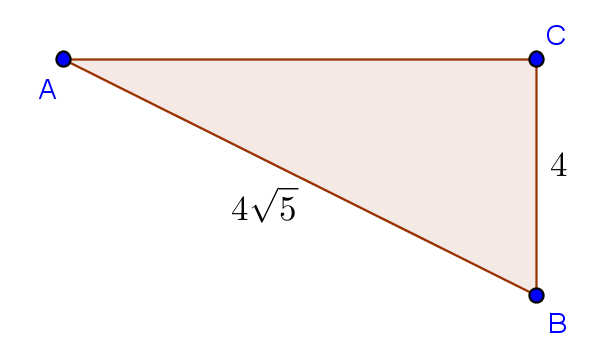
\includegraphics[width=0.3\textwidth]{10}
\ep

\bp{23}
다음 그림의 삼각형에서 \(\angle B\)의 삼각비를 각각 구하여라.\\
(1) \(\sin A\) =\\
(2) \(\cos A\) =\\
(3) \(\tan A\) =
\par\center
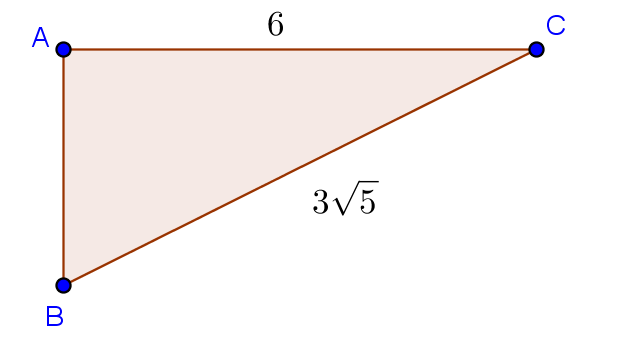
\includegraphics[width=0.3\textwidth]{11}
\ep

\bp{24}
다음 그림의 삼각형에서 \(\angle A\)의 삼각비를 각각 구하여라.\\
(1) \(\sin A\) =\\
(2) \(\cos A\) =\\
(3) \(\tan A\) =
\par\center
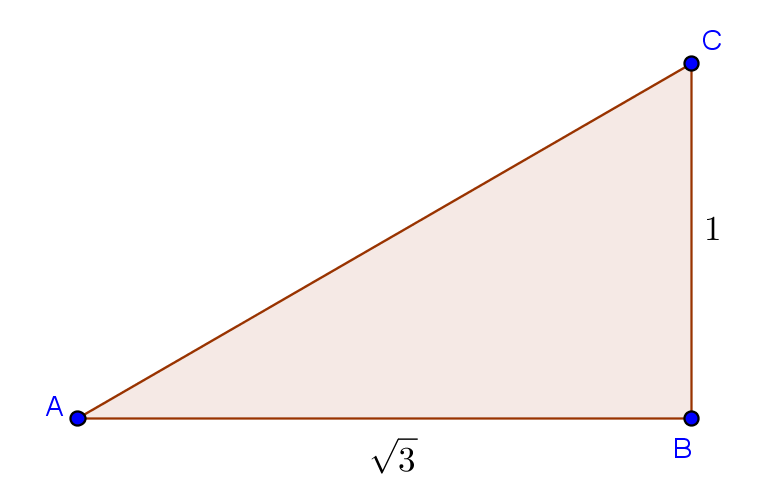
\includegraphics[width=0.3\textwidth]{12}
\ep

\bp{25}
다음 그림의 삼각형에서 \(\angle A\)의 삼각비를 각각 구하여라.\\
(1) \(\sin A\) =\\
(2) \(\cos A\) =\\
(3) \(\tan A\) =
\par\center
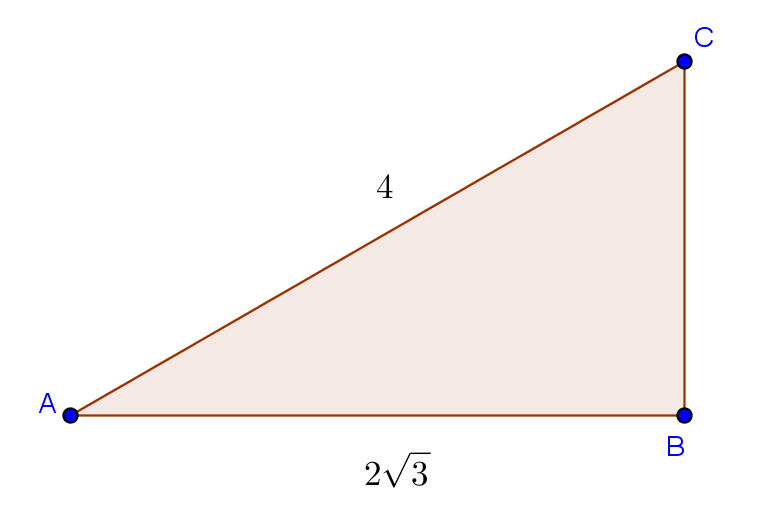
\includegraphics[width=0.3\textwidth]{13}
\ep

\bp{26}
다음 그림의 삼각형에서 \(\angle C\)의 삼각비를 각각 구하여라.\\
(1) \(\sin A\) =\\
(2) \(\cos A\) =\\
(3) \(\tan A\) =
\par\center
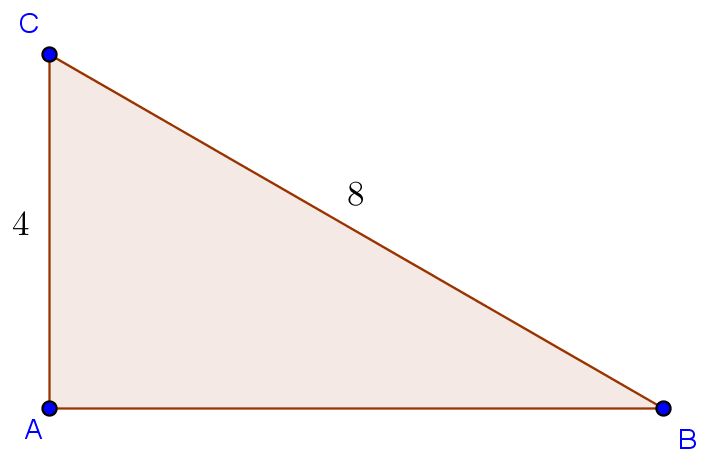
\includegraphics[width=0.3\textwidth]{14}
\ep

%\newpage
%\section*{답}
%01 : \(48\)\\
%02 : \(54\)\\
%03 : \\
%04 : \(48\)\\
%05 : 
\end{document}